\documentclass[a4paper,11pt]{article}
\usepackage{amsmath,amsthm,amsfonts,amssymb,amscd,amstext,vmargin,graphics,graphicx,tabularx,multicol} \usepackage[french]{babel}
\usepackage[utf8]{inputenc}  
\usepackage[T1]{fontenc} 
\usepackage[T1]{fontenc}
\usepackage{amsmath,amssymb}
\usepackage{pstricks-add,tikz,tkz-tab,variations}
\usepackage[autolanguage,np]{numprint} 

\setmarginsrb{1.5cm}{0.5cm}{1cm}{0.5cm}{0cm}{0cm}{0cm}{0cm} %Gauche, haut, droite, haut
\newcounter{numexo}
\newcommand{\exo}[1]{\stepcounter{numexo}\noindent{\bf Exercice~\thenumexo} : \marginpar{\hfill /#1}}
\reversemarginpar


\newcounter{enumtabi}
\newcounter{enumtaba}
\newcommand{\q}{\stepcounter{enumtabi} \theenumtabi.  }
\newcommand{\qa}{\stepcounter{enumtaba} (\alph{enumtaba}) }
\newcommand{\initq}{\setcounter{enumtabi}{0}}
\newcommand{\initqa}{\setcounter{enumtaba}{0}}

\newcommand{\be}{\begin{enumerate}}
\newcommand{\ee}{\end{enumerate}}
\newcommand{\bi}{\begin{itemize}}
\newcommand{\ei}{\end{itemize}}
\newcommand{\bp}{\begin{pspicture*}}
\newcommand{\ep}{\end{pspicture*}}
\newcommand{\bt}{\begin{tabular}}
\newcommand{\et}{\end{tabular}}
\renewcommand{\tabularxcolumn}[1]{>{\centering}m{#1}} %(colonne m{} centrée, au lieu de p par défault) 
\newcommand{\tnl}{\tabularnewline}

\newcommand{\trait}{\noindent \rule{\linewidth}{0.2mm}}
\newcommand{\hs}[1]{\hspace{#1}}
\newcommand{\vs}[1]{\vspace{#1}}

\newcommand{\N}{\mathbb{N}}
\newcommand{\Z}{\mathbb{Z}}
\newcommand{\R}{\mathbb{R}}
\newcommand{\C}{\mathbb{C}}
\newcommand{\Dcal}{\mathcal{D}}
\newcommand{\Ccal}{\mathcal{C}}
\newcommand{\mc}{\mathcal}

\newcommand{\vect}[1]{\overrightarrow{#1}}
\newcommand{\ds}{\displaystyle}
\newcommand{\eq}{\quad \Leftrightarrow \quad}
\newcommand{\vecti}{\vec{\imath}}
\newcommand{\vectj}{\vec{\jmath}}
\newcommand{\Oij}{(O;\vec{\imath}, \vec{\jmath})}
\newcommand{\OIJ}{(O;I,J)}

\newcommand{\bmul}[1]{\begin{multicols}{#1}}
\newcommand{\emul}{\end{multicols}}


\newcommand{\reponse}[1][1]{%
\multido{}{#1}{\makebox[\linewidth]{\rule[0pt]{0pt}{20pt}\dotfill}
}}

\newcommand{\titre}[5] 
% #1: titre #2: haut gauche #3: bas gauche #4: haut droite #5: bas droite
{
\noindent #2 \hfill #4 \\
#3 \hfill #5

\vspace{-1.6cm}

\begin{center}\rule{6cm}{0.5mm}\end{center}
\vspace{0.2cm}
\begin{center}{\large{\textbf{#1}}}\end{center}
\begin{center}\rule{6cm}{0.5mm}\end{center}
}



\begin{document}
\pagestyle{empty}
\titre{Contrôle de Mathématiques }{Nom :}{Prénom :}{Classe}{Date}


\exo{4}

\q Donner la définition d'un parallélogramme.\\


\q Tracer le quadrilatère KLMN pour que KLMN soit un parallélogramme de centre O et le parallélogramme NSPH.

\bmul{2}


\begin{flushleft}
\includegraphics[scale=0.8]{para.eps} 

\end{flushleft}

\columnbreak



\emul

\bmul{2}
\q Nommer quatre parallélogrammes dans la figure ci-contre, 
en sachant que :  (AH)$\slash\slash$(CJ) ; (BG) $\slash\slash$(DI) ; (AD)$\slash\slash$(EF)$\slash\slash$(GJ)  :

\columnbreak

\includegraphics[scale=1]{fig1.eps} 

\emul

\exo{3} 

\bmul{2}

\initq
\q Le quadrilatère BLEU est un parallélogramme. Quel est la mesure de l'angle $\widehat{BLE}$ ? (Une démonstration est attendue)

\columnbreak
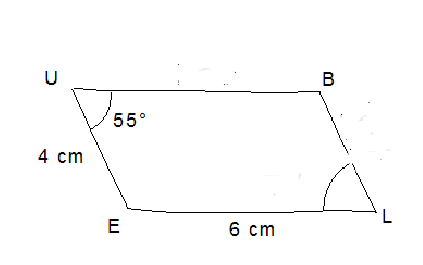
\includegraphics[scale=0.8]{demo1.eps} 

\emul


\bmul{2}
\q Quel est la mesure de la longueur IO? (Une démonstration est attendue)


\columnbreak
\includegraphics[scale=1]{demo2.eps} 

\emul


 
\exo{2,5} 

\bmul{2}
\initq \q Démontrer que le quadrilatère ci-contre est un parallélogramme.\\

\q Quel est la mesure de l'angle $\widehat{LMG}$ ?\\

\columnbreak

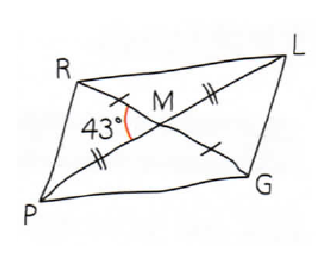
\includegraphics[scale=1]{fig2.eps} 

\emul
										


 \newpage

\exo{2} Dire si l'affirmation est vraie ou fausse 	\\

\qa Tout parallélogramme a un axe de symétrie : .....................\\

\qa Un parallélogramme peut avoir un angle de 28\degre et un angle de 62\degre : ...................\\

\qa Si LYNX est un parallélogramme, alors LX = YN : ...................\\

\qa Si CHAT est un parallélogramme de centre O, alors les triangles COH et AOT ont le même périmètre :.......................\\


\exo{2}
Les tableaux suivants sont-ils des tableaux de proportionnalité ? (Justifier votre réponse)\\


\bmul{2}

\initqa \qa \begin{tabular}{|c|c|c|}
\hline 
\hspace*{0.2cm}1\hspace*{0.2cm} & \hspace*{0.2cm}2\hspace*{0.2cm} &\hspace*{0.2cm} 3 \hspace*{0.2cm}\\ 
\hline 
 \hspace*{0.2cm}3\hspace*{0.2cm} & \hspace*{0.2cm}4 &\hspace*{0.2cm} 5 \hspace*{0.2cm}\\ 
\hline 
\end{tabular} 

\columnbreak

\qa \begin{tabular}{|c|c|c|}
\hline 
\hspace*{0.2cm}8\hspace*{0.2cm} & \hspace*{0.2cm}12 \hspace*{0.2cm}& \hspace*{0.2cm}20 \hspace*{0.2cm}\\ 
\hline 
\hspace*{0.2cm} 88\hspace*{0.2cm}& \hspace*{0.2cm}132\hspace*{0.2cm} &\hspace*{0.2cm} 220 \hspace*{0.2cm}\\ 
\hline 
\end{tabular} 

\emul

\medskip

\exo{2}
Compléter sur le sujet les tableaux de proportionnalité suivants :\\

\bmul{2}

\begin{tabular}{|c|c|c|c|}
\hline 
Soda (mL) & \hspace*{0.2cm}1000\hspace*{0.2cm} & \hspace*{0.2cm}100\hspace*{0.2cm} &\hspace*{0.2cm}  \\ 
\hline 
Nombre de sucre & \hspace*{0.2cm}25\hspace*{0.2cm} & \hspace*{0.2cm} &\hspace*{0.2cm} 55 \\ 
\hline 
\end{tabular} 

\columnbreak

\begin{tabular}{|c|c|c|c|}
\hline 
Temps (en min) &\hspace*{0.2cm}12\hspace*{0.2cm} & \hspace*{0.2cm}15 \hspace*{0.2cm}& \hspace*{0.2cm}20 \\ 
\hline 
Distance (en m) &\hspace*{0.2cm} & \hspace*{0.2cm}90\hspace*{0.2cm} &\hspace*{0.2cm}  \\ 
\hline 
\end{tabular} 

\emul

\medskip

\exo{2}

Le robinet d'un lavabo fuit, il perd 10 cL d'eau par minute.\\

\noindent \initq \q Quelle quantité d'eau, en cL, s'écoule en une heure ?\\
\q Quelle quantité d'eau, en cL, s'écoule en une journée ?\\
\q Combien de temps faudra-t-il pour que 1 $m^{3}$ se soit écoulé de ce robinet ? (On rappelle que 1 $m^{3}$ = 1 000L)\\

\medskip

\exo{2,5}

En jouant aux fléchettes, Ilan marque 10 points quand il touche la cible et il perd 4 points quand il la rate. Ilan a 182 points, mais il ne se souvient plus combien de fois il a visé la cible.\\

\noindent \initq \q Que représentent $x$ et $y$ ?\\
\q Vérifier qu'il est possible que $x=25$ et $y=17$. Dans ce cas, combien de fois Ilan a-t-il pu viser la cible ?\\



\end{document}
